\chapter{Results}
\label{chap:results}

\section{Cohort and Data Availability}

This section describes cohort composition, scar morphology heterogeneity across the
105 valid cases, and available clinical metadata.

\subsection{Scar morphology and inter-patient heterogeneity}
\label{sec:scarmorph}

Visual inspection of the full-cohort 3D grid confirmed that all 105 cases produce
geometrically coherent LV reconstructions with identifiable core-zone surfaces. Beyond
confirming quality, the grid reveals the amplitude of scar morphology present in this cohort.
Scar extent ranges from small, focal lesions occupying a single wall segment to large,
multi-territory scars covering a substantial fraction of the myocardium. Spatial organisation
varies from compact, contiguous surfaces to fragmented geometries with disconnected
components distributed across different wall regions. Infarction location spans all three coronary territories (LAD, RCA, LCX)---with scar
affecting inferior, anterior, lateral, and septal walls---at basal, mid-ventricular, and
apical levels, with variable wall-depth involvement from subendocardial to near-transmural.
This degree of heterogeneity is a defining characteristic of the cohort and directly motivates
the need for a shape representation that makes no assumptions about scar location, extent,
or connectivity.

\subsection{Clinical metadata and demographic profile}

Cross-referencing the DEVELOP registry CSV (173 records, 88 with segmentation flag) with
the geometrically valid cases yields 48 patients with usable age and sex labels. Among
these, 38 are male (79.2\%), mean age $63.0 \pm 11.5$ years (median 63.0, IQR 54.8--72.0).
The high missingness of demographic and outcome variables makes supervised clinical
outcome modelling infeasible; all geometric analyses proceed on the full 105-case cohort.

\section{Polar Map Construction and Orientation Verification}

This section reports pipeline performance across the 105-case cohort: apex detection
outcomes, projection method consistency, grid resolution sensitivity, and comparison
against a reference flattening method.

\subsection{Apex and axis detection}

The multi-candidate apex detection strategy (Section~\ref{sec:polarmaps}) was applied
to all 105 cases. LV~PC1 was selected as the apex-defining direction in 74\% of cases,
RV~PC1 in 21\%, and LV~PC2 in the remaining 5\% (Figure~\ref{fig:apexdirection}). In
the RV~PC1 cases, LV~PC1 aligned with circumferential rather than longitudinal variance,
producing an incorrect apex location shifted toward the lateral wall (the free wall of the
left ventricle facing away from the septum, in the direction opposite to the right ventricle). In the LV~PC2 cases,
near-equal variance in the two largest dimensions caused the true long axis to be captured
by the second rather than the first principal direction. The multi-candidate strategy correctly
identified the apical tip in all 105 cases.

A forced-LV-PC1 ablation confirmed that constraining the axis to LV~PC1 regardless of
eccentricity produces incorrect apex detection in the 25\% of cases where RV~PC1 or
LV~PC2 would otherwise be selected, demonstrating that a single fixed direction is
insufficient for this cohort (Figure~\ref{fig:app_axis_winner} in Appendix). A qualitative
comparison against the reference flattening method of N\'{u}\~{n}ez Garc\'{i}a
\cite{nunez2018} is presented in Section~\ref{sec:polarmapverif}.

\begin{figure}[ht]
    \centering
    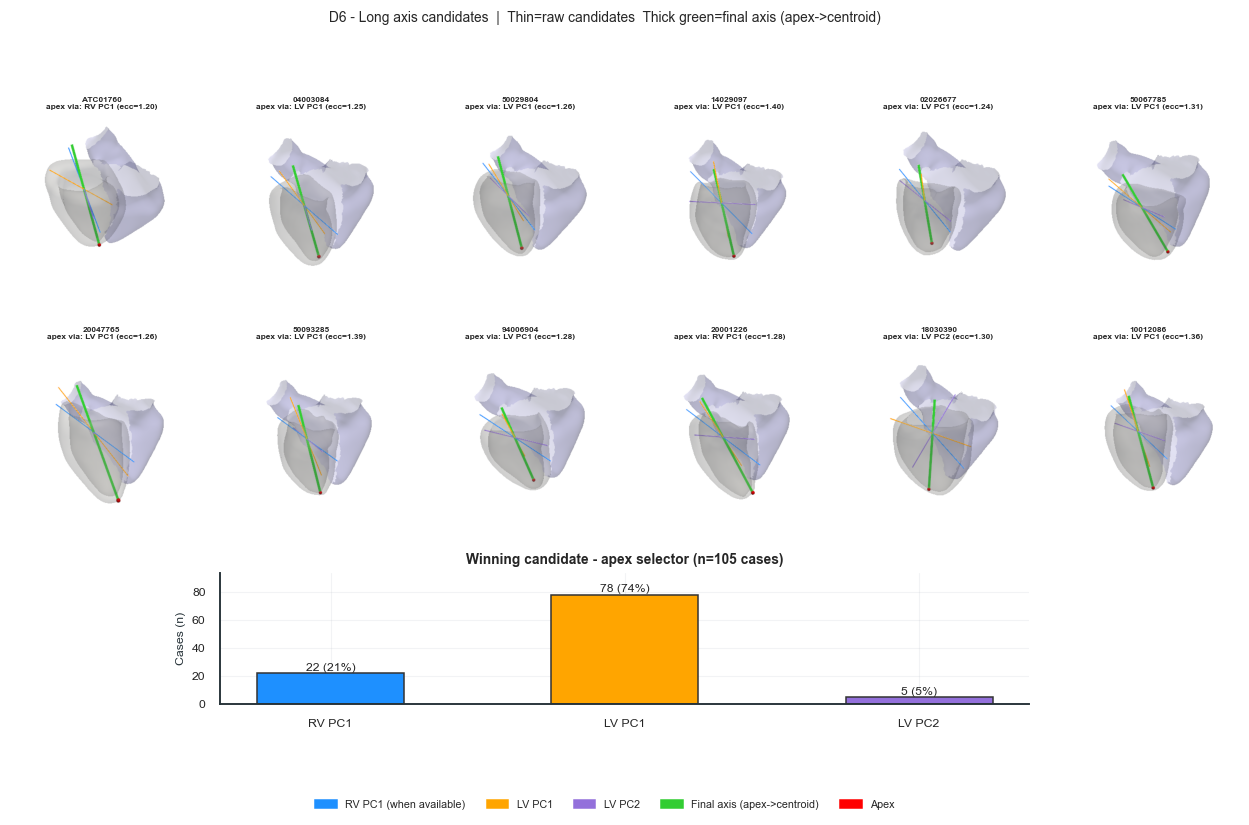
\includegraphics[width=0.68\textwidth]{figures/d6_long_axis_candidates}
    \caption{Apex-defining direction selected per patient ($n=105$): LV~PC1 in 74\%, RV~PC1 in 21\%, LV~PC2 in 5\%.}
    \label{fig:apexdirection}
\end{figure}

\vspace{-0.8em}
\subsection{Projection method comparison}
\label{sec:projmethods}

Three complementary projection methods were evaluated at the population level: the
vertex-based method (binary scar presence per polar bin), the area-based method
(projected core-zone surface area in mm$^2$ per bin), and the coverage method
(core-zone area divided by total LV area per bin). The spatial pattern of scar concentration is consistent across methods: all three identify
the same high-burden regions and the same low-burden regions, with differences confined
to relative intensity rather than spatial location. Population-level superposition maps for
all three methods are shown in Figure~\ref{fig:superposition}.

\begin{figure}[H]
    \centering
    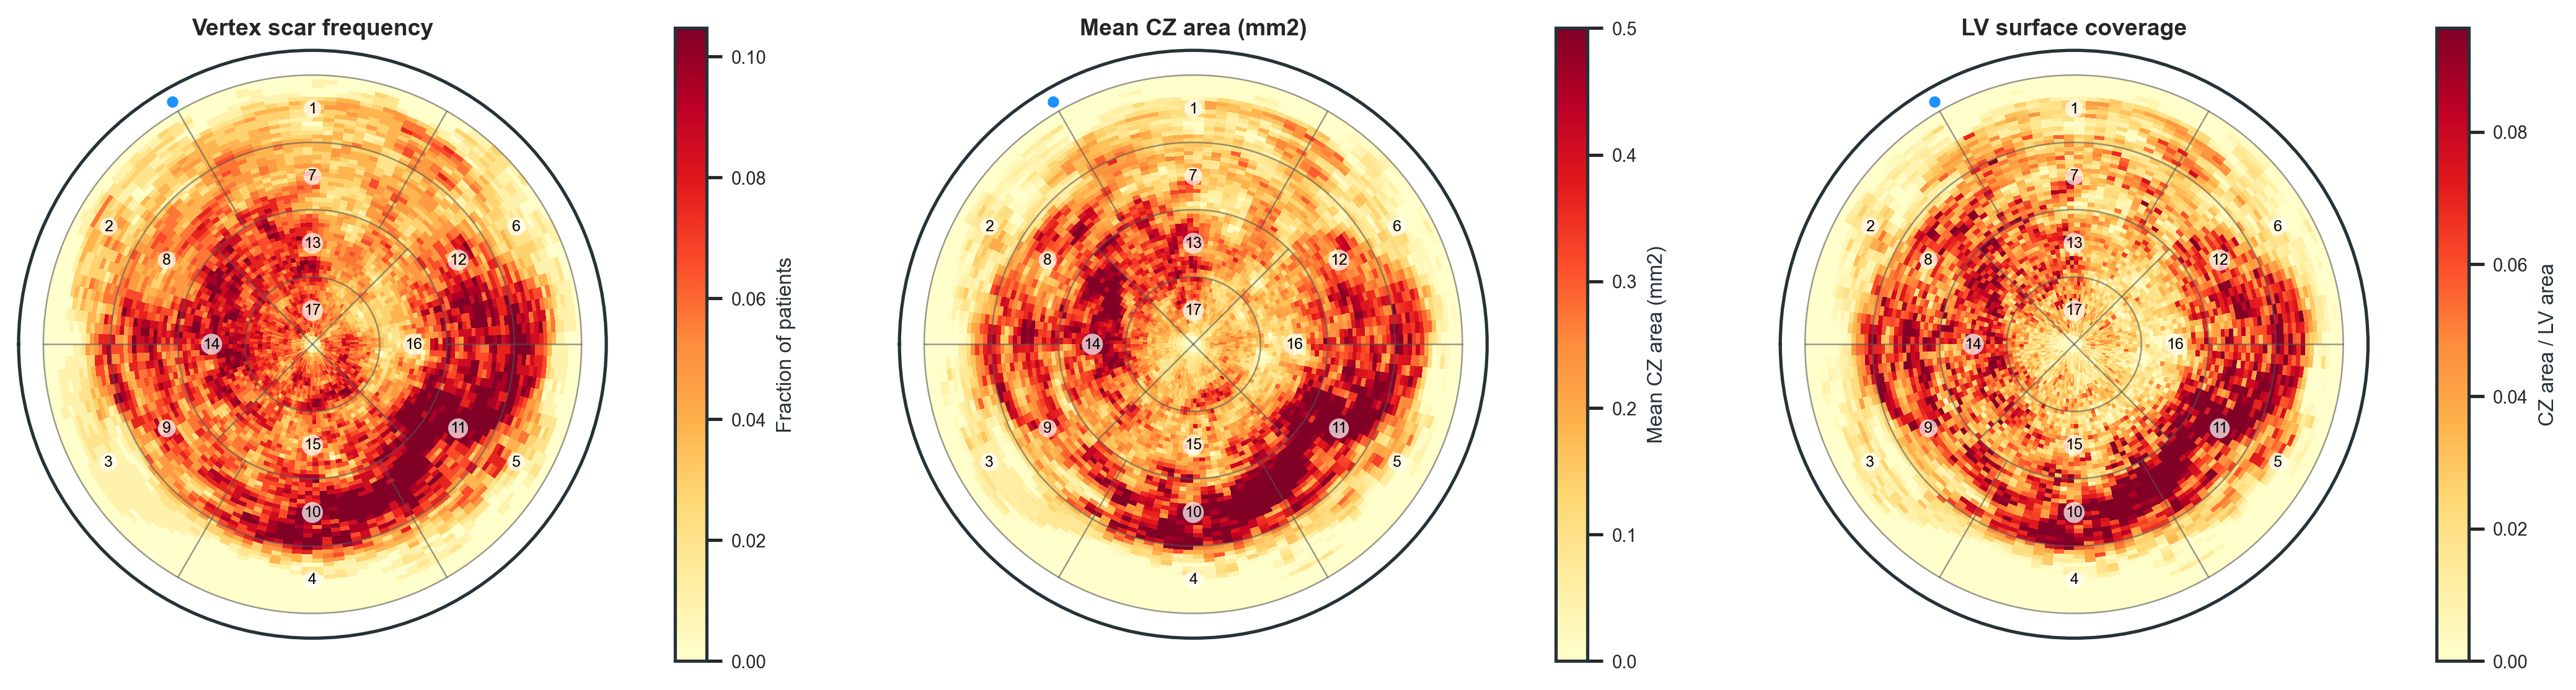
\includegraphics[width=\textwidth]{figures/fig3_population_superposition}
    \caption{Population superposition maps ($n=105$) for vertex-based, area-based, and LV coverage methods. Spatial patterns are consistent; the coverage method reveals higher RCA density obscured in vertex-based by that territory's smaller surface area.}
    \label{fig:superposition}
\end{figure}

\subsection{Grid resolution sensitivity}

The operational $64 \times 128$ polar grid was compared against a coarser ($32 \times 64$)
and a finer ($128 \times 256$) alternative. The three configurations differ substantially in
their vertex density per bin (Table~\ref{tab:grid}).

\begin{table}[htbp]
    \centering
    \caption{Grid resolution comparison.}
    \label{tab:grid}
    \begin{tabular}{lrr}
        \toprule
        Grid & Bins & Avg.\ LV vertices/bin \\
        \midrule
        $32 \times 64$ (coarse) & 2\,048 & ${\sim}24$ \\
        $64 \times 128$ (operational) & 8\,192 & ${\sim}6$ \\
        $128 \times 256$ (fine) & 32\,768 & ${\sim}1.5$ \\
        \bottomrule
    \end{tabular}
\end{table}

The $64 \times 128$ grid provides the best trade-off: ${\sim}6$ vertices per bin gives stable
binary scar detection with sufficient resolution to distinguish all 17 AHA segments. Population
mean maps are consistent across all three resolutions (Figure~\ref{fig:app_gridres} in Appendix).

\subsection{Verification of polar maps}
\label{sec:polarmapverif}

Visual inspection of representative cases shows that scar localisation is broadly consistent
between the two methods in both circumferential and longitudinal coordinates. The primary
discrepancy concerns radial density: the $r^{1/3}$ radial displacement applied by the
reference method concentrates scar representations toward the basal ring, whereas the
linear mapping used here distributes coverage more uniformly along the apex-to-base axis;
as a consequence, the proposed method recovers scar points near the apex with greater
completeness. The 3D LV reconstruction and polar map comparison for the representative case are shown in
Figure~\ref{fig:verif_combined}. More generally, the longitudinal coordinate $s$ of the
proposed method encodes apex-to-base position directly as the normalised projection onto
the long axis, providing a monotonic and geometrically interpretable representation of the
full apex-to-base gradient; the flat disk radius of the reference method is determined by the
conformal (angle-preserving) flattening transformation, whose output depends on the global
geometry of the endocardial surface and cannot be expressed as a simple function of
normalised apex-to-base position alone.
Cross-referencing with the 3D LV shell further suggests that the two methods sample
different transmural depths: the reference method labels endocardial surface points in
proximity to the Core Surface and therefore captures the endocardial face of the scar,
whereas the proposed method projects Core Surface vertices directly and therefore
represents the full transmural extent of the scar mass. Taken together, the two approaches
are complementary: differences in radial density and transmural sampling reflect distinct
mapping choices rather than errors in anatomical localisation.

\begin{figure}[ht]
    \centering
    \begin{subfigure}[b]{0.33\textwidth}
        \centering
        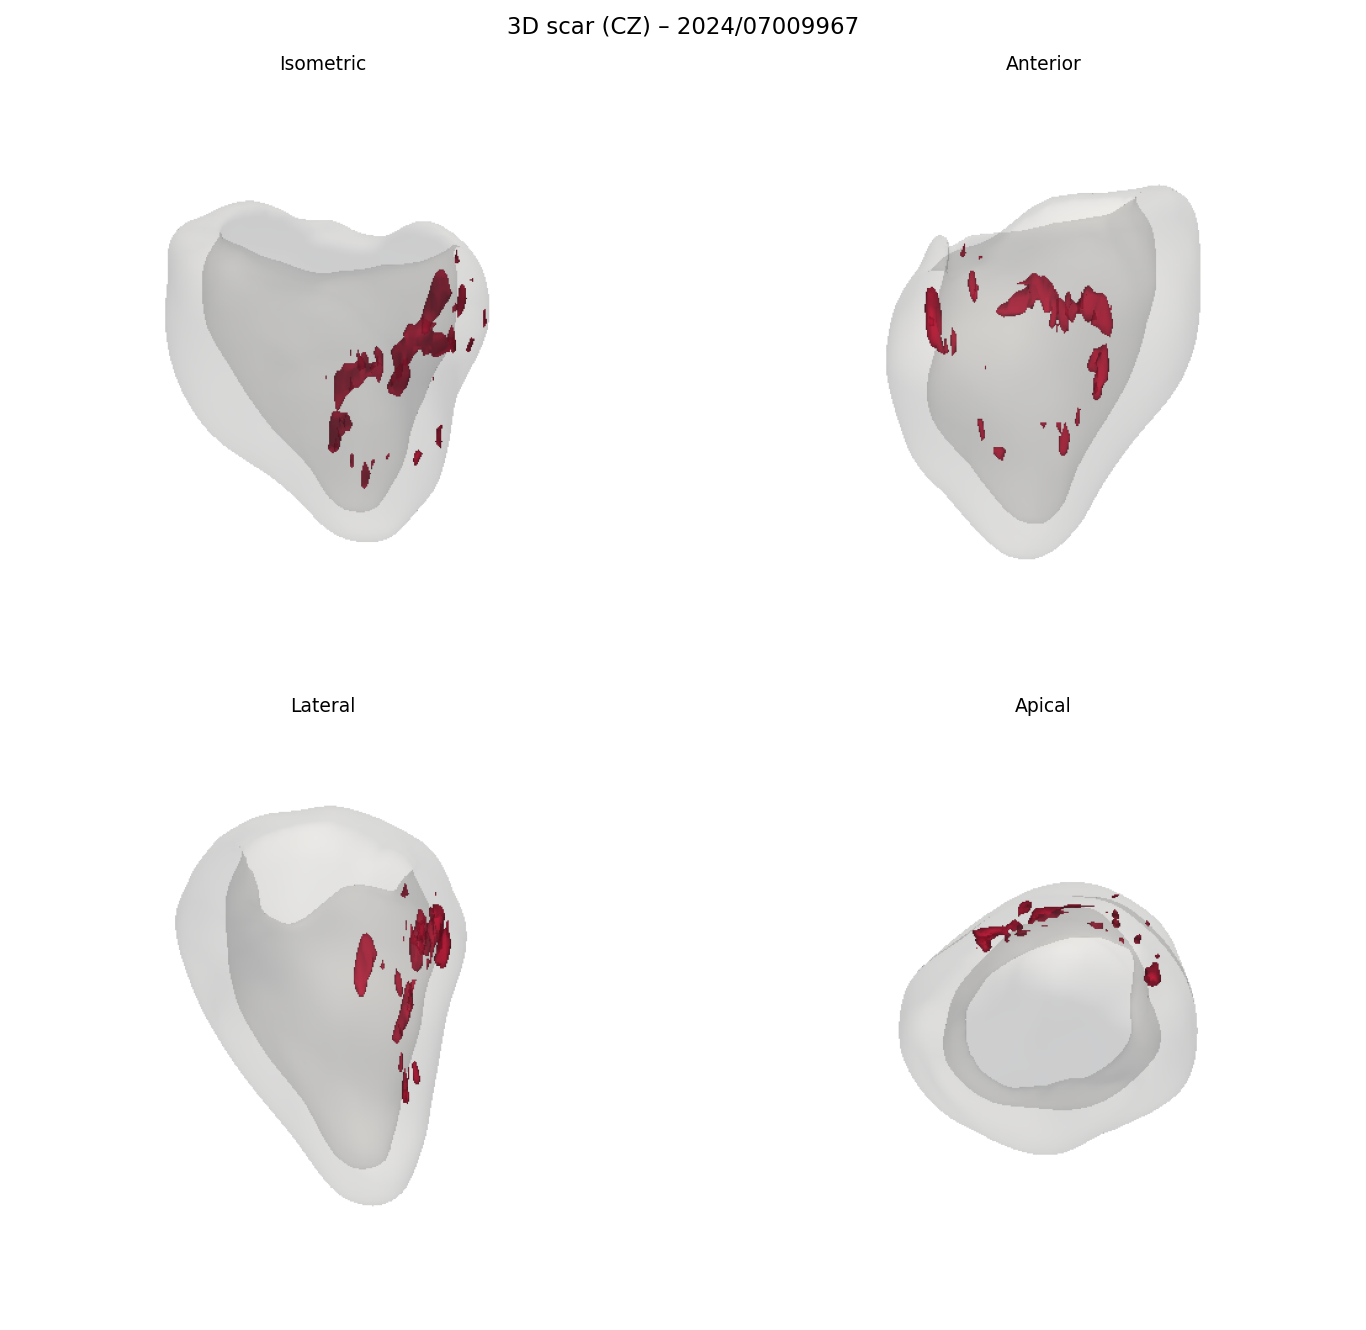
\includegraphics[width=\textwidth]{figures/M06_3d_scar_2024_07009967}
    \end{subfigure}
    \hfill
    \begin{subfigure}[b]{0.52\textwidth}
        \centering
        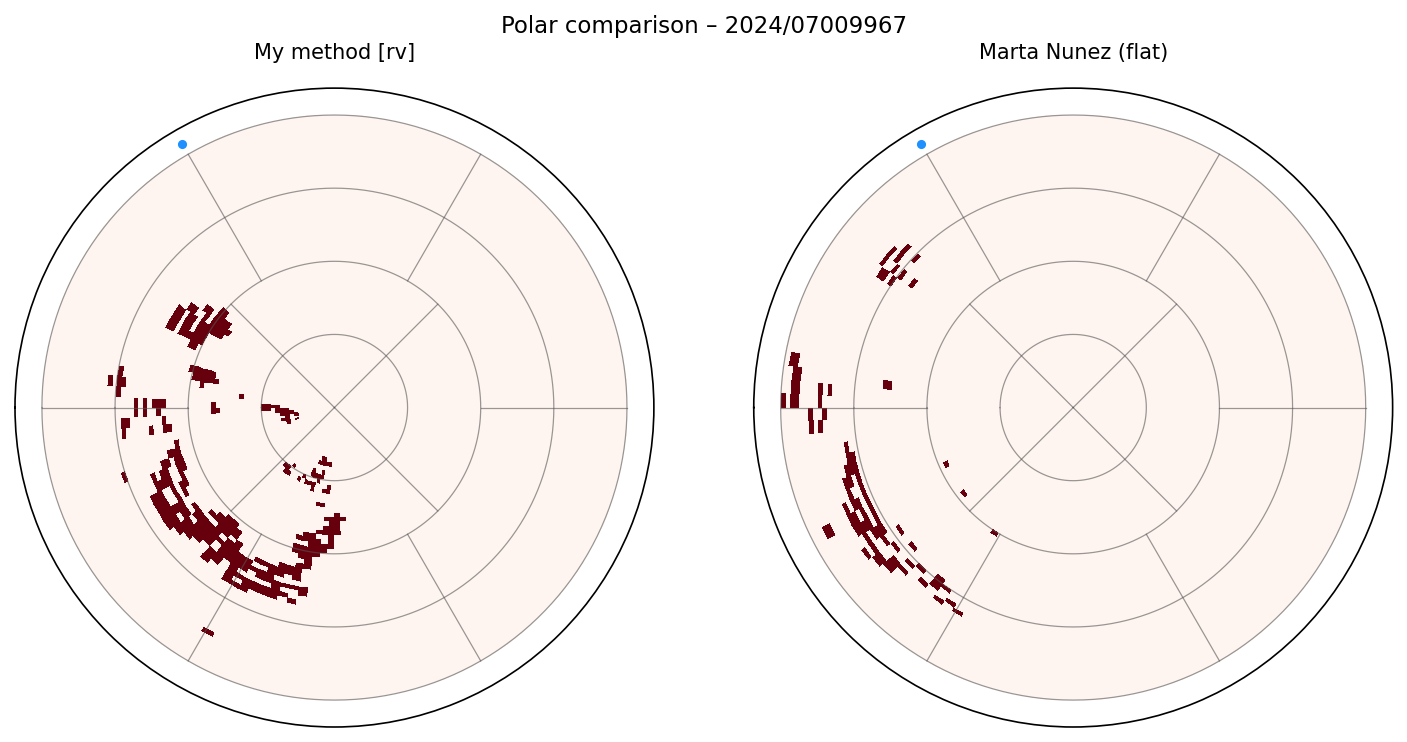
\includegraphics[width=\textwidth]{figures/M06_polar_comparison_2024_07009967}
    \end{subfigure}
    \caption{Verification for case 2024\_07009967: (a) 3D LV with core-zone scar (red); (b) polar map comparison, proposed method (left) vs.\ N\'{u}\~{n}ez Garc\'{i}a \cite{nunez2018} (right). Scar localisation is consistent; differences reflect distinct mapping choices.}
    \label{fig:verif_combined}
\end{figure}

\FloatBarrier
\section{Population-Level Scar Analysis}

All analyses used vertex-based binary polar maps on the full 105-case cohort with
non-parametric methods, as justified by the normality diagnostics below.

\subsection{Normality diagnostics}

Univariate normality was assessed via QQ plots, comparing the Pearson correlation
between sample and theoretical normal quantiles against critical values at $\alpha = 0.05$.
Only age satisfied the normality criterion. Since univariate normality is a necessary
condition for multivariate normality, the failure of all scar-related variables precludes a
multivariate normal joint distribution analytically; a chi-squared QQ plot of squared
Mahalanobis distances of the full 17-segment burden vector was computed to corroborate
this visually.

All scar-related variables showed strong zero-inflation and right skewness: at the AHA
segment level, 70--75\% of patients had zero scar in most segments, with mean/median
ratios of 2.4--3.7 and SD/mean ratios of 2--4. Territory-level and global burden variables
showed similar patterns, with less extreme zero-inflation due to bin aggregation. All
subsequent analyses therefore used non-parametric methods (Friedman test, Wilcoxon
signed-rank, Spearman rank correlation) and patient-level bootstrap confidence intervals
(2\,000 resamples).

\subsection{AHA-17 segment burden and population atlas}

A notable structural property of the segment-level distributions is the dissociation between
prevalence and extent: a segment can be frequently affected yet carry low mean burden, or
rarely affected but carrying high conditional burden when it is. This arises directly from
zero-inflation---the unconditional mean is dragged toward zero even when the conditional
mean among affected patients is substantial. Segment-level summaries therefore report both
quantities separately. For example, the basal inferolateral segment (seg 5) is scar-positive
in 44.8\% of patients yet carries an unconditional mean burden of only 0.032, because the
majority of patients contribute a zero; the apical septal segment (seg 14) is affected in a
similar proportion of patients (41.0\%) but, when involved, carries a conditional mean burden
of 0.190---nearly six times higher.

The Friedman test confirmed that scar burden is non-uniformly distributed across the 17 AHA
segments within patients ($p = 3.3 \times 10^{-17}$, $n = 105$). Although
this result is anatomically expected---ischaemic infarction follows coronary territory
boundaries, making uniform distribution implausible a priori---the formal test establishes that
the data are internally consistent with anatomical priors. Post-hoc pairwise Wilcoxon signed-rank tests with
Bonferroni correction (136 comparisons, adjusted threshold $\alpha = 0.000368$) identified
20 segment pairs with statistically significant burden differences. The significant pairs were
not distributed uniformly across the LV: they were concentrated between the inferior and
inferoseptal mid-ventricular segments (segments 9--11) and the anterior basal segments
(segments 1--4), with mid inferior (segment 10) and mid inferolateral (segment 11) emerging
as the segments most consistently distinguishable from the rest of the wall. No significant
differences were found among segments within the same anatomical ring (i.e.\ segments
sharing the same apex-to-base level, such as the six basal segments 1--6) or between
neighbouring segments in the lateral basal region, where scar burden values were similarly
low across adjacent sectors, indicating that the spatial heterogeneity is structured rather
than diffuse: the significant pairwise differences are not scattered randomly across the 136
comparisons but concentrate specifically between the inferior mid-ventricular segments
(10--11, highest burden) and the anterior basal segments (1--4, lowest burden), a pattern
consistent with the anatomical boundaries of the RCA and LAD territories.

Bootstrap confidence intervals confirm a statistically robust spatial hierarchy. Basal
segments (1--4, mean 0.014--0.023) are clearly and reliably spared: their CI upper bounds
($\leq 0.035$) do not overlap with the CI lower bounds of the mid-cavity hotspot segments
(segs 10--11, CI lower $\geq 0.061$). The mid-inferolateral segment (seg 11, mean = 0.100,
95\% CI [0.070, 0.135]) is the single most affected region, followed by the mid-inferior
(seg 10, mean = 0.088) and apical septal (seg 14, mean = 0.078) segments. The wide CIs
of hotspot segments reflect the high inter-patient variability driven by zero-inflated,
right-skewed distributions. The population atlas identifies a robust inferior-to-apical hotspot
centred on the mid-inferolateral and mid-inferior segments (AHA 11 and 10), straddling the
RCA--LCX boundary, with basal segments consistently spared.

% [FIGURE PLACEHOLDER --- archetype/atlas map to be inserted]
The bootstrap population mean polar map is provided in Appendix~\ref{app:atlas}.

\subsection{Coronary territory burden and archetype maps}
\label{sec:terrburden}

The 2\% threshold for territory involvement was selected via sensitivity analysis across
candidate values (1\%, 2\%, 3\%, 5\%, 10\%); the full sensitivity curve is shown in
Figure~\ref{fig:app_territory_threshold} in the Appendix. At 1\% the multi-territory fraction
exceeded 60\%, implausibly high for a focal-infarct cohort; thresholds above 3\%
progressively assigned no-scar classification to patients with minor genuine involvement.
The 2\% value represents the earliest stable point at which single-territory classification
reaches its plateau and the no-scar fraction remains low (${\sim}10\%$).

LCX showed the numerically highest mean territory burden (0.055), followed by LAD (0.051)
and RCA (0.047). These differences were not statistically significant ($p = 0.148$), indicating no systematic coronary territory preference at the
population level. Ring-level analysis showed that the apical and mid-cavity rings carry the
highest scar involvement, with the basal ring consistently spared.

Archetype maps stratified by dominant territory reveal distinct spatial geometries. LAD-dominant
scar is the most diffuse: it extends longitudinally from the anteroseptal segments down through
the apex (segment 17), producing an elongated pattern along the long axis that spans multiple
rings. RCA- and LCX-dominant scar, by contrast, tends toward circumferential spread at the
mid-cavity level, wrapping around the inferior and lateral walls with less longitudinal extension.
This difference reflects the anatomical territory boundaries: the LAD supplies the anterior wall
and apex, while RCA and LCX supply the inferior and lateral walls, which are arranged more
circumferentially in the mid-ventricular ring.

The lower vertex-based RCA burden does not imply geometrically insignificant infarction:
as shown by the coverage analysis (Section~\ref{sec:projmethods}), RCA scar tends to be
locally concentrated when present: the total scar surface area per bin classified as
scar-positive is higher for RCA than for LCX or LAD, meaning RCA scar packs more tissue
area into a smaller number of bins.

The area-based and vertex-based analyses produced concordant spatial rankings at both
segment and territory levels (Spearman $\rho > 0.85$ across all 17 segments and all three
territories), and both Friedman tests reached the same inferential conclusions, supporting
consistency across methodologically independent quantification approaches.

\subsection{Inter-segment correlation structure and PCA}

The $17 \times 17$ Spearman inter-segment correlation matrix reveals a block-diagonal
structure aligned with coronary territories: segments within the same territory co-vary
positively, consistent with shared vascular supply causing contiguous infarction. Importantly,
the dominant within-territory correlation pattern is longitudinal (apex-to-base) rather than
circumferential---vertically adjacent segments (e.g.\ seg 5 and seg 11, both LCX but at
different ring levels) show higher correlations than circumferentially adjacent segments in
different territories, indicating that scar penetrates transmurally along the wall depth rather
than spreading circumferentially. Inter-territory correlations are weak, with the smallest
observed between LCX and RCA ($\rho = 0.114$), supporting the treatment of territory
burdens as approximately independent dimensions.

PCA of the $z$-score standardised 17-segment vectors shows that six components are
needed to explain 72\% of the variance, with PC1 accounting for only 18\%. This low
concentration of variance in the first component indicates that no single spatial mode
dominates scar variability---the scar pattern space is intrinsically high-dimensional, reflecting
the diversity of infarct locations and extents across the cohort.

\subsection{Age and sex associations}

No segment reached significance after Bonferroni correction ($\alpha = 0.05/17$, $n = 48$).
Numerically strongest trends: mid-inferior seg~10 ($\rho = 0.345$, $p_\text{Bonf} = 0.280$)
and apex seg~17 ($\rho = -0.307$, $p_\text{Bonf} = 0.575$); RCA territory $\rho = 0.285$
($p = 0.050$, n.s.). Sex-stratified analysis was not performed due to severe imbalance
(38 male / 10 female).

\subsection{Transmurality}

Figure~\ref{fig:transmurality_combined} shows
fragment-level onset and transmurality stratified by ring zone and coronary territory. Onset measures the shallowest wall depth at which scar begins (0 =
endocardial, 1 = epicardial); transmurality is the span from onset to outermost depth. Both
are derived from the continuous vertex-depth computation described in
Section~\ref{sec:statistical}.

The continuous vertex-depth approach yields a mean fragment onset of 0.300 and a mean
fragment transmurality of 0.190, indicating that scar originates near the endocardial surface
and extends approximately 19\% of wall thickness---consistent with subendocardial ischaemic
infarction. Onset is lowest in the apical and mid rings and highest in the basal ring.
This is expected because coronary occlusions most commonly occur at mid-artery levels;
the ischaemic wavefront propagates from the occluded segment outward, reaching basal
myocardium last and with reduced severity, so scar there tends to begin deeper in the wall.
By coronary territory, RCA presents the highest onset (mean 0.318) and the highest
transmurality (mean 0.216), making it the most deeply penetrating territory in this cohort.

The transmurality gradient analysis shows a positive population-mean core-to-edge
difference, confirming a dense-core / thin-edge transmural structure: the central scar mass
extends more deeply through the wall than its periphery.

Endocardial dominance was confirmed at the cohort level: on average 65\% of scar-positive
bins per patient showed onset $\leq 30\%$ of wall thickness (endocardial), 20\% fell in the
midwall range (30--60\%), and 15\% showed epicardial-dominant onset ($> 60\%$).

\begin{figure}[htbp]
    \centering
    \begin{subfigure}[t]{0.48\textwidth}
        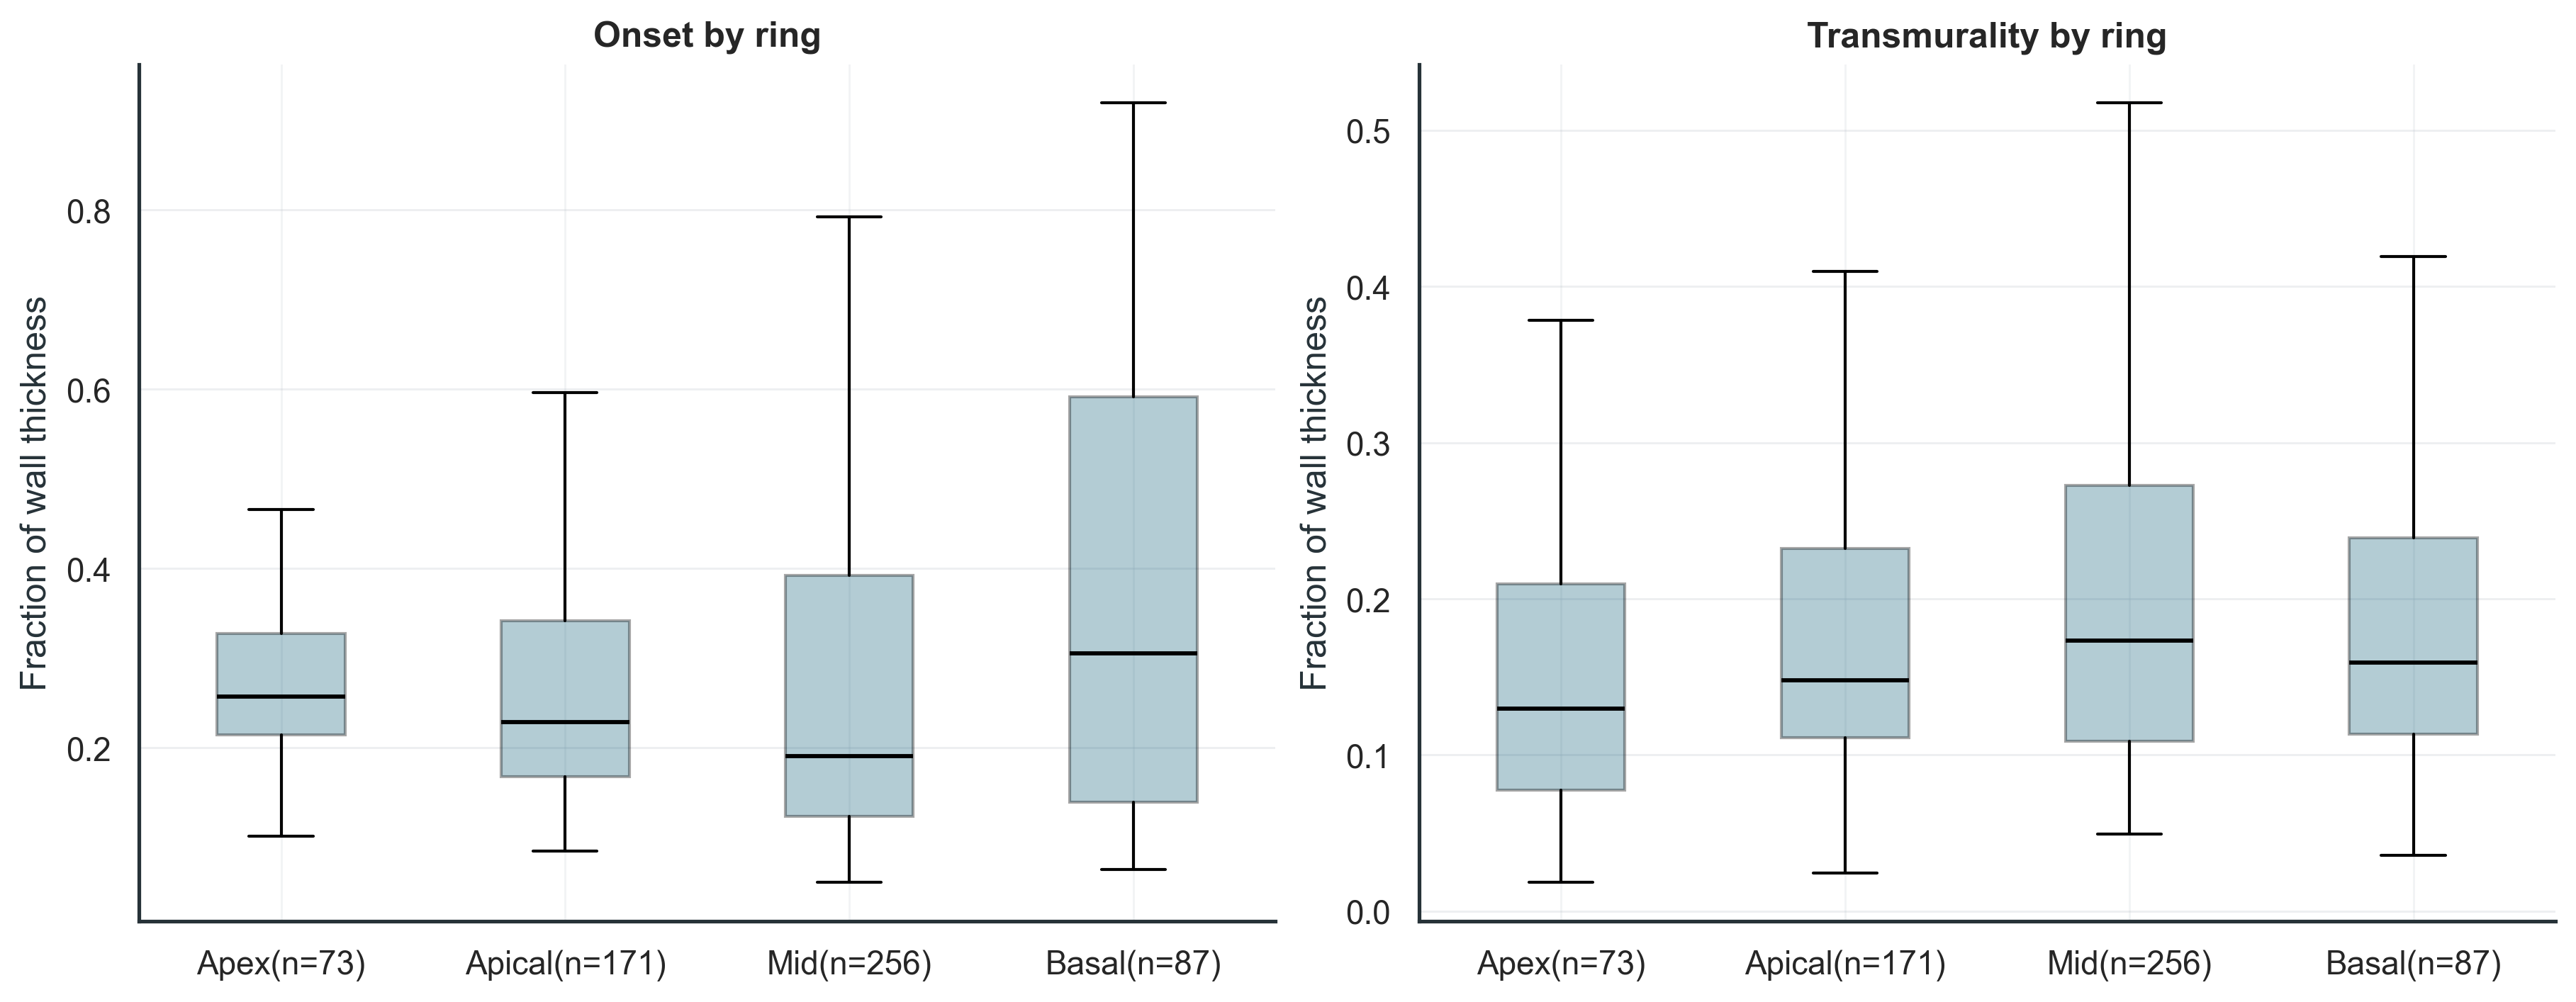
\includegraphics[width=\textwidth]{figures/fragment_onset_transmurality_by_ring}
    \end{subfigure}
    \hfill
    \begin{subfigure}[t]{0.48\textwidth}
        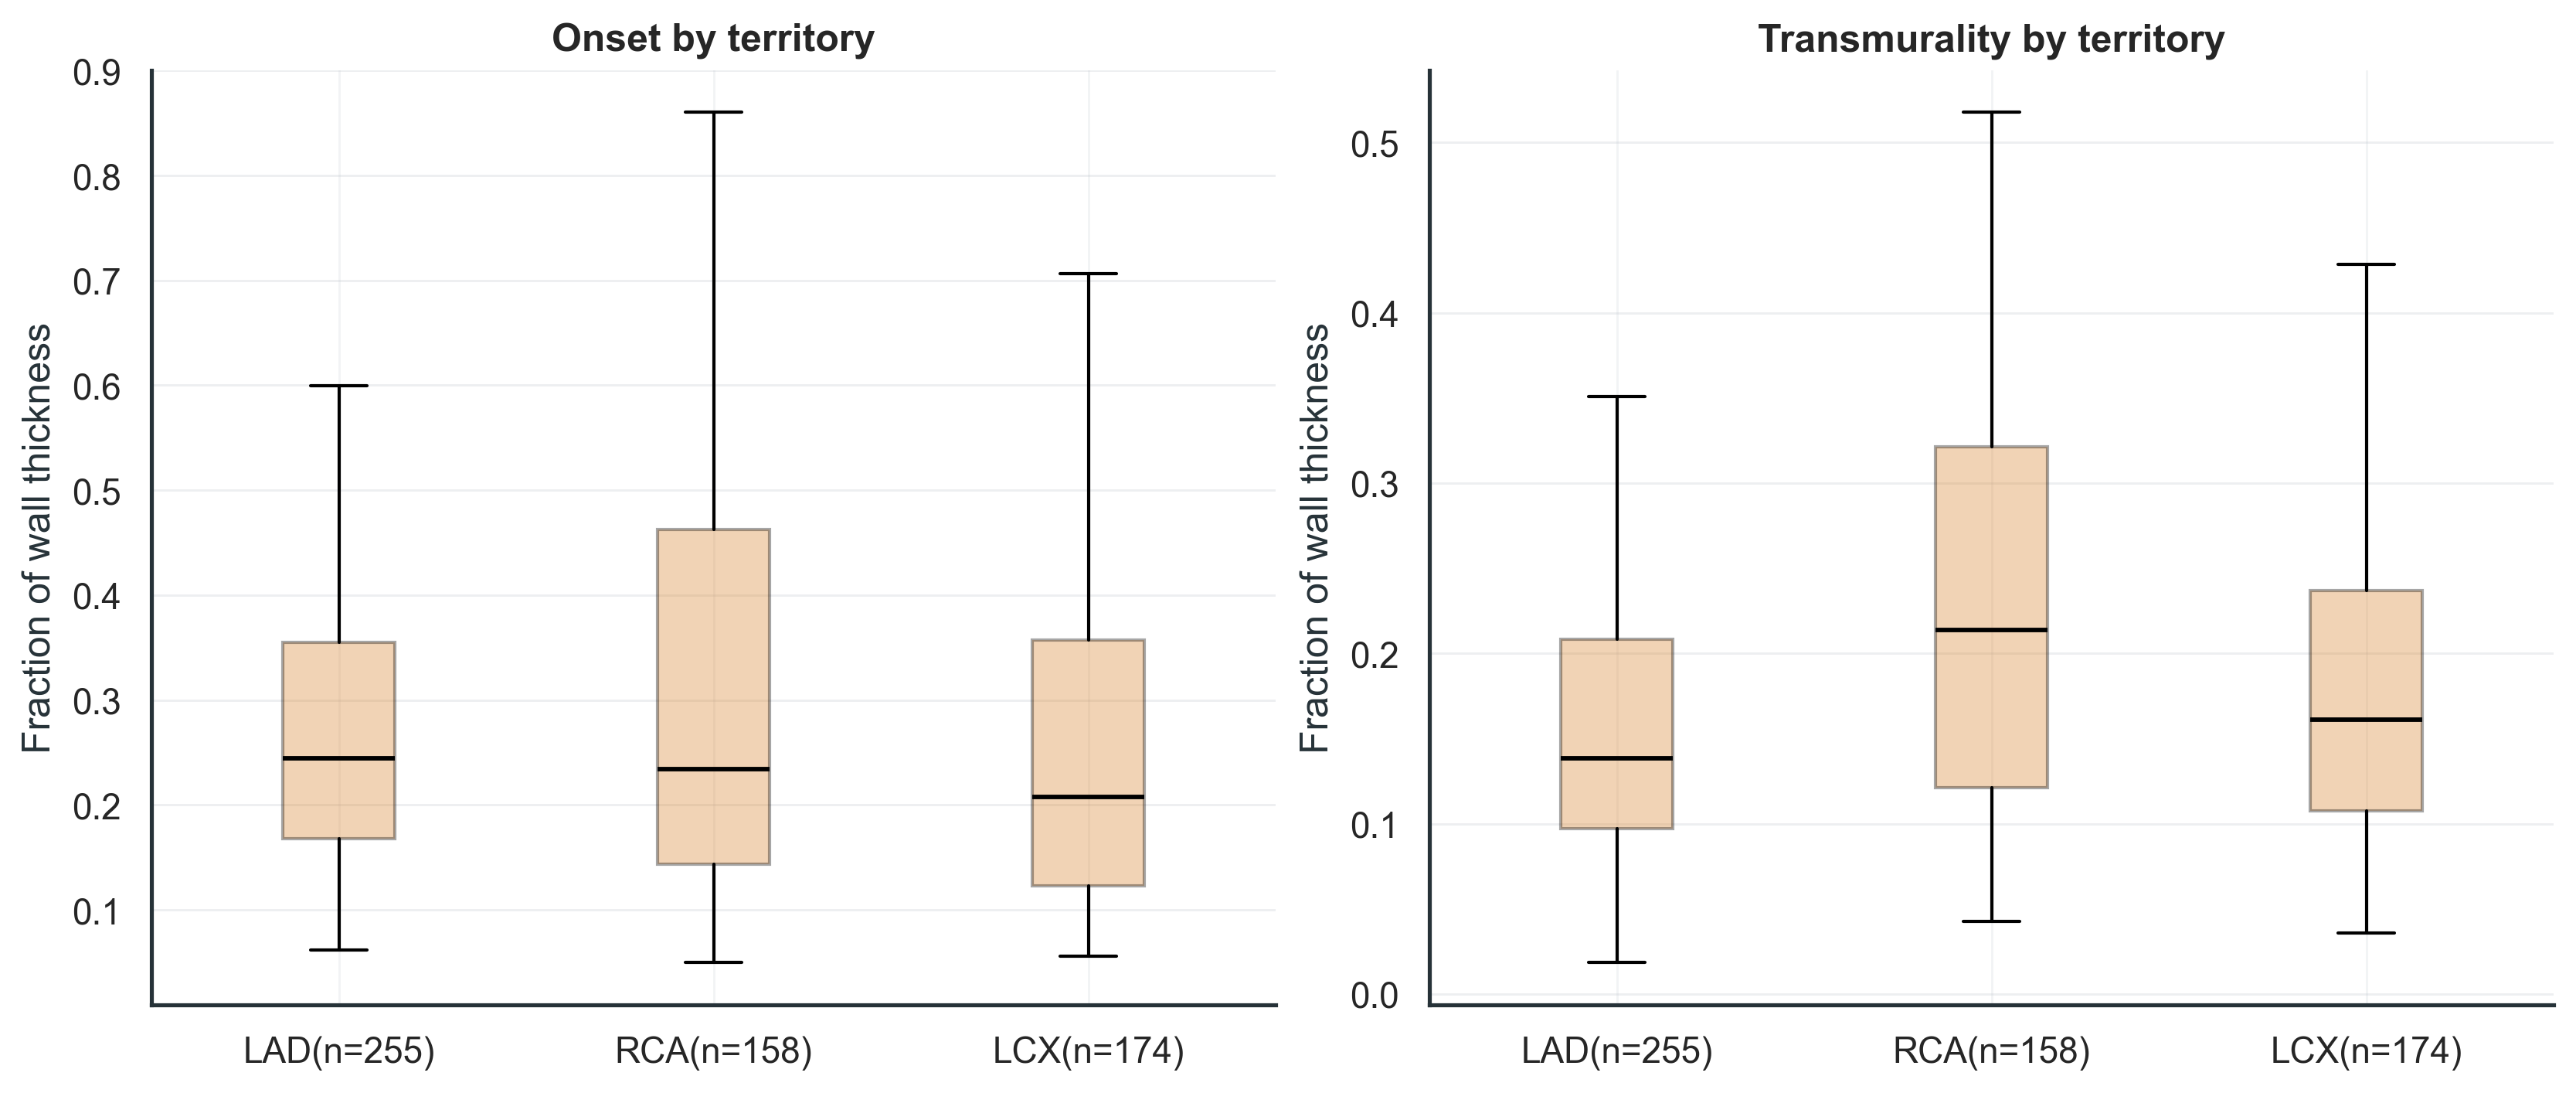
\includegraphics[width=\textwidth]{figures/fragment_onset_transmurality_by_territory}
    \end{subfigure}
    \caption{Fragment-level onset and transmurality stratified by (a) ring zone and (b) coronary territory.
    Onset = shallowest wall depth at which scar begins (0 = endocardial, 1 = epicardial);
    transmurality = span from onset to outermost depth, both derived from the continuous
    vertex-depth method (Section~\ref{sec:statistical}).}
    \label{fig:transmurality_combined}
\end{figure}

\vspace{-0.8em}
\subsection{Geometric descriptors and fragment shape}

Within-patient Spearman correlation between the 17-element segment-level extent vector
and the 17-element per-segment mean transmurality vector yielded a median $\rho = 0.571$
(mean 0.547, IQR [0.359, 0.800]; $n = 97$ patients with computable correlation, i.e.\ at
least three AHA segments with both valid transmurality and positive scar extent; the
remaining 8 patients had insufficient scar-positive segments for a valid rank correlation),
confirming partial but incomplete association: in most patients more-burdened segments
tend to penetrate more deeply, but the relationship is far from deterministic.

The apex-to-base scar gradient showed near-zero population means (linear slope:
$-0.031 \pm 0.165$; Spearman $\rho$: $+0.088 \pm 0.425$) with extreme inter-patient
variability: slopes ranged from $-0.82$ (strongly apex-dominant) to $+0.20$ (base-dominant),
and $\rho$ from $-0.89$ to $+0.74$. When averaged across the cohort, no dominant
longitudinal preference is detected by the apex-to-base gradient analysis; however, at the
individual level the gradient discriminates strongly between apex-dominant and base-dominant
patterns, and other analyses---notably the territory archetype maps---do reveal longitudinal
differences once patients are stratified by coronary territory.

Shape analysis of the largest scar fragment showed that most patients present irregular,
non-compact lesions (median compactness 0.39). The mid ring is where scar appears most
circumferentially spread.

\FloatBarrier
\section{Retrieval-Based Scar Generation}

This section reports the leave-one-out retrieval evaluation: feature vector comparison,
distance metric selection, and performance statistics under deterministic and probabilistic
modes.

\subsection{Feature vector comparison and selection}

Six candidate descriptor vectors were evaluated under leave-one-out retrieval with Manhattan
distance. Table~\ref{tab:featurevectors} and Figure~\ref{fig:featurevectors} report their
dimensionality and the three retrieval quality metrics. SVD scree plots and patient PC1--PC2
scatter plots for all vectors are provided in Figure~\ref{fig:app_svd_plots} in the Appendix.

\begin{table}[htbp]
    \centering
    \caption{Leave-one-out (LOO) retrieval performance, six descriptor vectors (Manhattan distance, $n=105$). Mean and median $|\Delta\text{CZ}|$ lower is better; Seg/Polar Dice higher is better.}
    \label{tab:featurevectors}
    \small
    \begin{tabular}{lrrrrrr}
        \toprule
        Vector & Feats & Mean $|\Delta\text{CZ}|$ & Med $|\Delta\text{CZ}|$ & Seg Dice & Polar Dice \\
        \midrule
        \textbf{full}        & \textbf{39} & 0.0148 & 0.0093 & \textbf{0.597} & 0.106 \\
        full\_no\_seg        & 22 & \textbf{0.0130} & \textbf{0.0079} & 0.489 & 0.100 \\
        full\_pruned         & 29 & 0.0188 & 0.0105 & 0.545 & 0.109 \\
        full\_ns\_pruned     & 16 & 0.0189 & 0.0115 & 0.474 & 0.093 \\
        pmap\_only           &  8 & 0.0188 & 0.0087 & 0.359 & \textbf{0.214} \\
        full\_ns+pmap        & 30 & 0.0136 & 0.0076 & 0.484 & 0.155 \\
        \bottomrule
    \end{tabular}
\end{table}

\begin{figure}[tb]
    \centering
    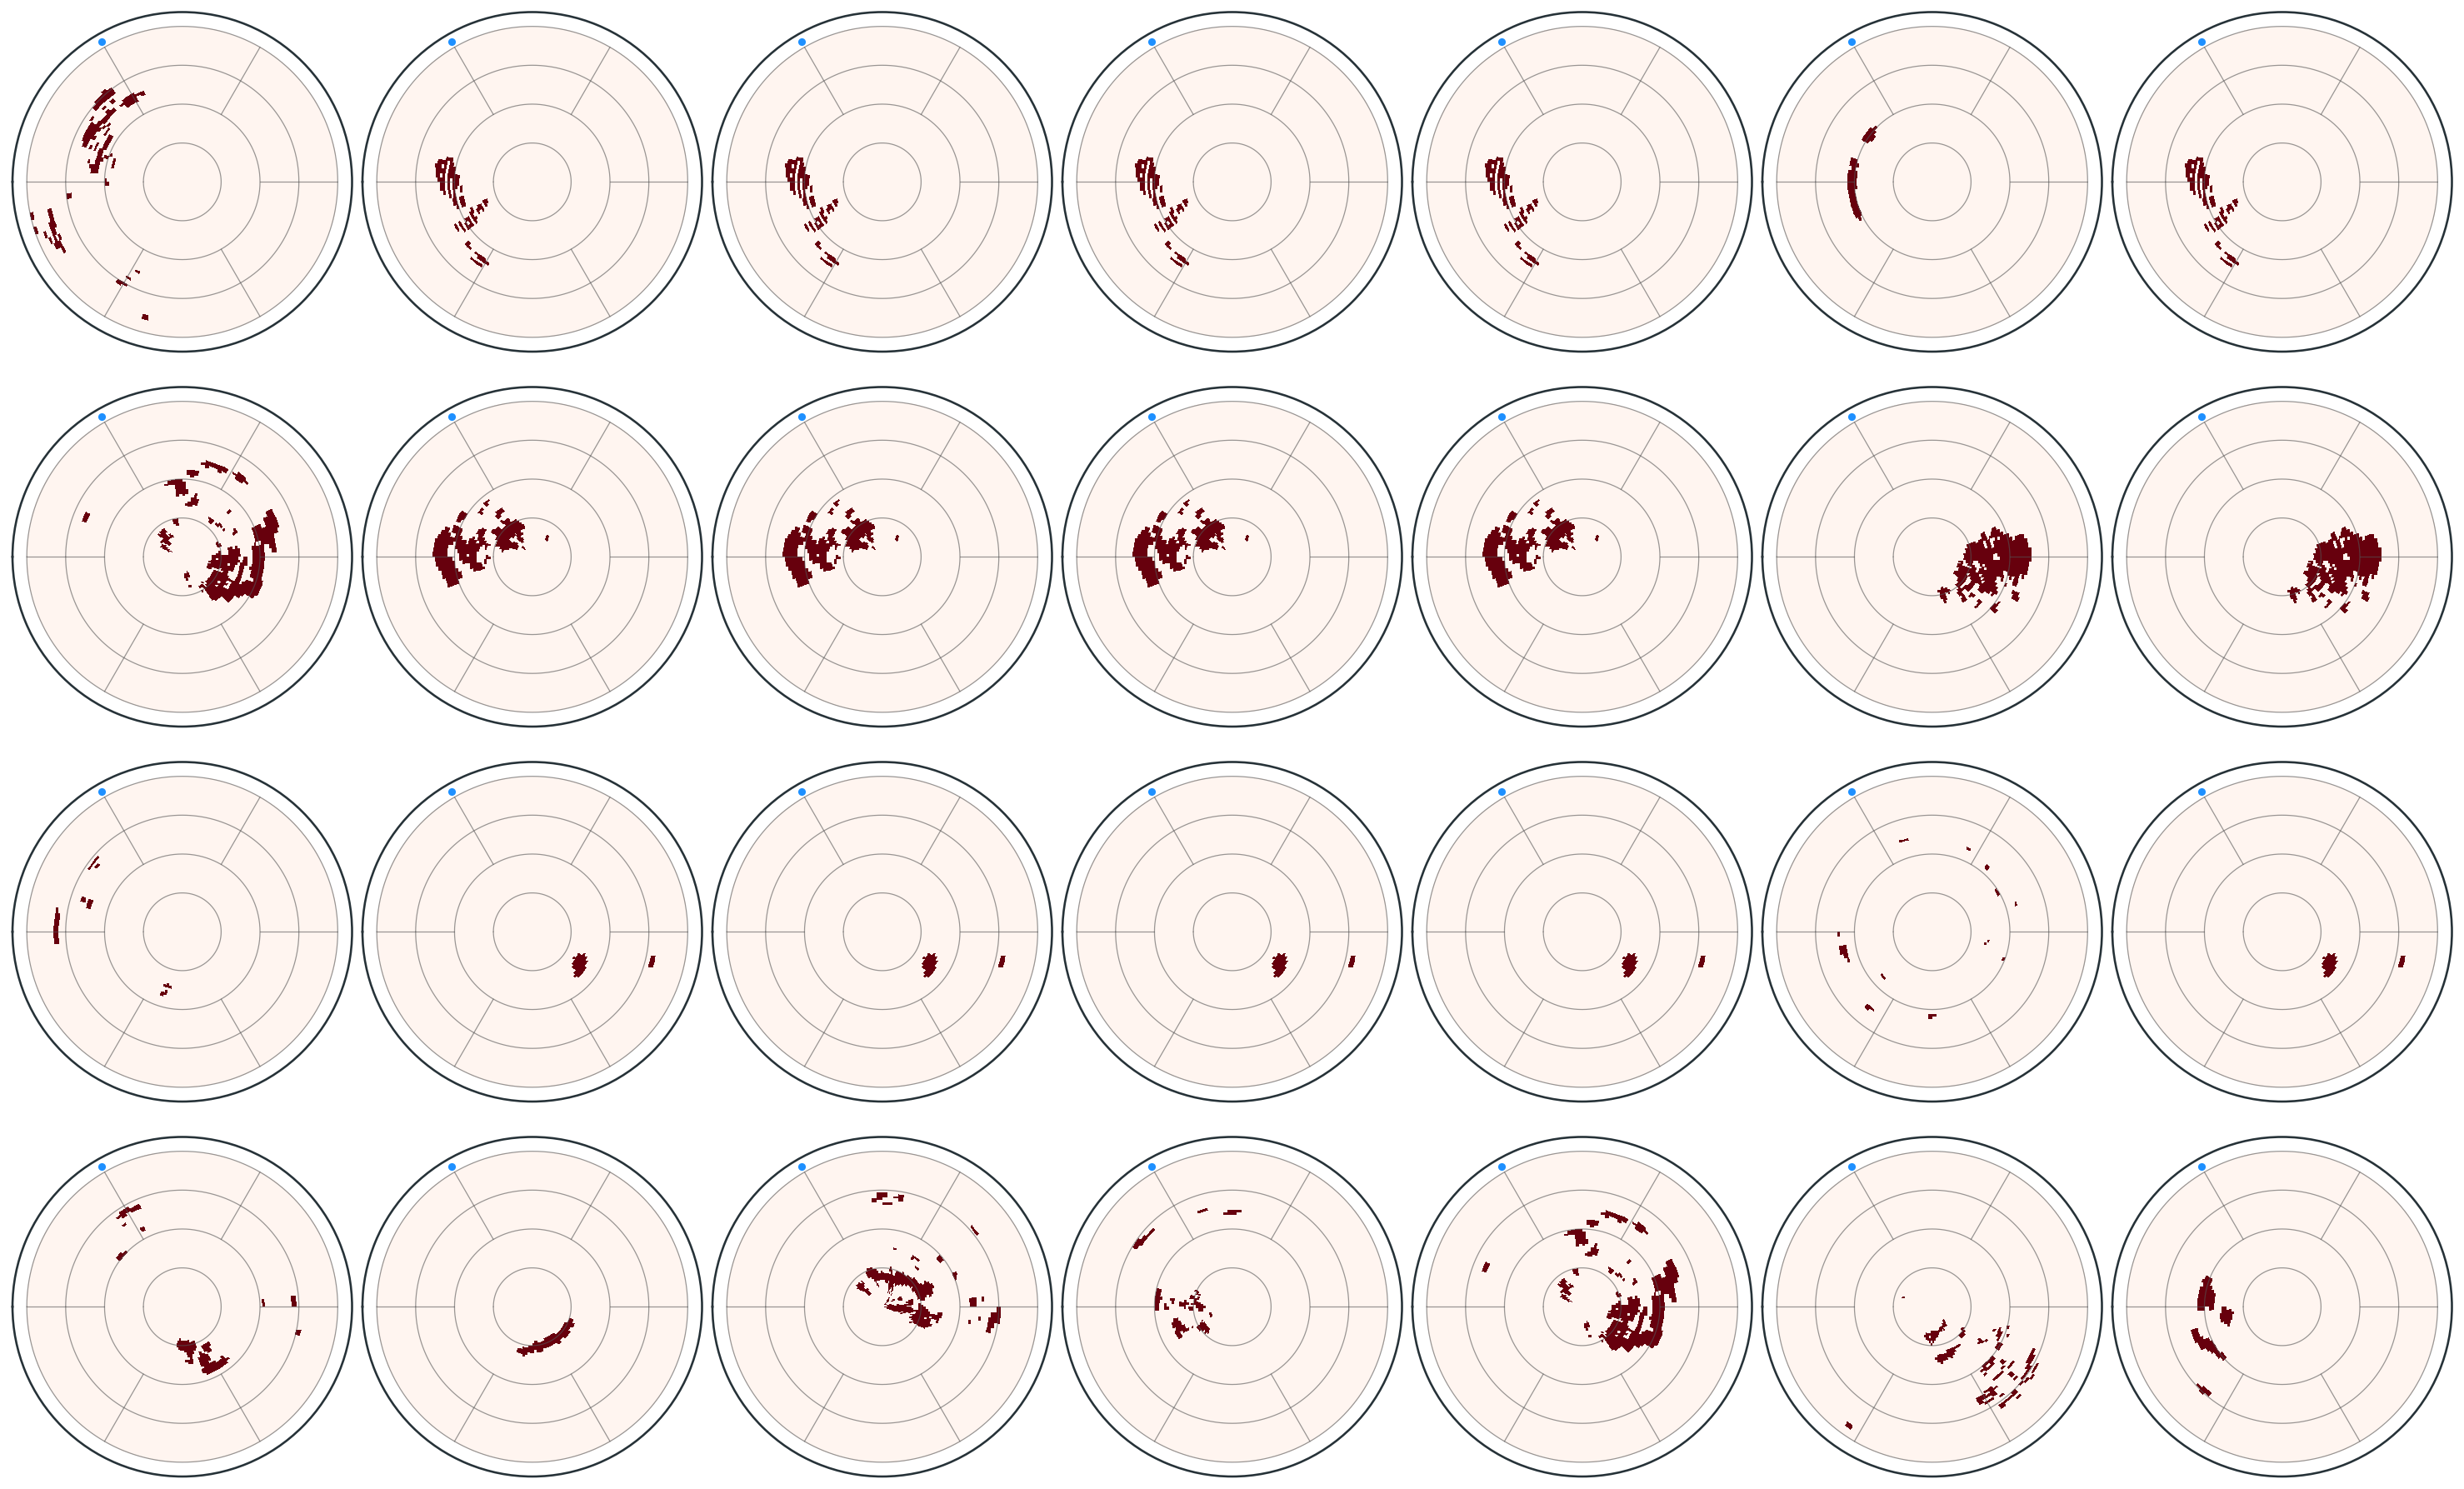
\includegraphics[width=0.80\textwidth]{figures/retrieval_six_vectors}
    \caption{Leave-one-out (LOO) retrieval performance for seven descriptor vectors
    (Manhattan distance, $n=105$). Columns from left to right: (1) target patient;
    (2)~\texttt{full} (39 features, all structured descriptors including AHA segment burdens);
    (3)~\texttt{full\_no\_seg} (22 features, structured descriptors without per-segment burdens);
    (4)~\texttt{full\_pruned} (29 features, \texttt{full} after SVD-based pruning);
    (5)~\texttt{full\_ns\_pruned} (16 features, \texttt{full\_no\_seg} after pruning);
    (6)~\texttt{pmap\_only} (8 features, principal component analysis (PCA) scores of binary polar maps);
    (7)~\texttt{full\_ns+pmap} (30 features, non-segment structured descriptors combined with polar-map PCA scores).}
    \label{fig:featurevectors}
\end{figure}

SVD analysis showed AHA segment features dominate variance (16 vs.\ 11 components for
90\% coverage in the segment-free variant). Feature pruning degraded performance on two
of three metrics (burden error 0.015$\to$0.019; segment Dice 0.597$\to$0.545), indicating
discriminative information is distributed across low-variance dimensions.
\textbf{pmap\_only} achieved highest polar-map Dice (0.214) but lowest segment Dice (0.359)
and worst burden error. The full 39-feature vector achieved the best segment-level Dice and
was selected as the primary descriptor because segment-level anatomical overlap was
prioritised and the features remain interpretable. However, it did not achieve the best value
on every metric: \textbf{full\_no\_seg} had the lowest scar burden error (0.0130
vs.\ 0.0148), and \textbf{pmap\_only} achieved the highest polar-map Dice (0.214
vs.\ 0.106). This shows that descriptor choice depends on the intended retrieval target.

\vspace{-0.8em}
\subsection{Distance metric comparison}

Manhattan distance on $z$-score normalised features outperformed Euclidean (segment Dice
0.597 vs.\ 0.539) and substantially outperformed cosine (segment Dice 0.282), which is
insensitive to vector magnitude.

\subsection{Performance on Territories and Deterministic and Probabilistic Retrieval}

Retrieval performance varied systematically by dominant coronary territory
(Table~\ref{tab:terrperf}): LCX-dominant patients achieved the lowest burden error
(mean $|\Delta\text{CZ}| = 0.010$) and highest segment Dice (0.629), followed by RCA
(0.013, 0.612) and LAD (0.023, 0.518). LAD-dominant scar---which extends longitudinally
across multiple rings---is harder to match than the more circumferentially localised RCA
and LCX patterns.

\begin{table}[htbp]
    \centering
    \caption{Leave-one-out (LOO) retrieval performance by dominant coronary territory and number of involved
    territories (full vector, Manhattan distance, $n=105$). $|\Delta\text{CZ}|$ = absolute core-zone (CZ) burden error;
    Seg Dice = segment-level Dice overlap over the AHA 17-segment model;
    Polar Dice = pixel-level overlap on the $64\times128$ polar grid.}
    \label{tab:terrperf}
    \small
    \begin{tabular}{lrrrr}
        \toprule
        Group & $n$ & Mean $|\Delta\text{CZ}|$ & Seg Dice & Polar Dice \\
        \midrule
        \multicolumn{5}{l}{\textit{By dominant territory}} \\
        LAD (Anterior) & 33 & 0.023 & 0.518 & 0.171 \\
        RCA (Inferior) & 31 & 0.013 & 0.612 & 0.064 \\
        LCX (Lateral)  & 41 & 0.010 & 0.629 & 0.086 \\
        \midrule
        \multicolumn{5}{l}{\textit{By number of involved territories}} \\
        1 territory & 40 & 0.012 & 0.550 & 0.090 \\
        2 territories & 41 & 0.015 & 0.533 & 0.141 \\
        3 territories & 13 & 0.034 & 0.617 & 0.122 \\
        \bottomrule
    \end{tabular}
\end{table}

By number of involved territories, single-territory patients showed the lowest burden error
(0.012), consistent with better case-base coverage of focal patterns. Three-territory patients
showed the highest burden error (0.034), reflecting that diffuse multi-territory scar is rare
enough to lack close matches among the remaining 104 cases.

In practice, the softmax weights are strongly concentrated on the nearest neighbour when its
distance is substantially smaller than the second-nearest. This was observed for several
patients in the cohort, where the nearest neighbour received sampling probability close to
1.0, making the probabilistic and deterministic modes effectively equivalent for those cases.
For patients whose top-10 neighbours are more evenly spaced in descriptor space, the
probabilistic mode distributes weight across multiple candidates, allowing different plausible
scar patterns to be returned for the same query.

A quantitative comparison across all 105 patients showed that the deterministic mode
achieves marginally better mean retrieval quality on all three metrics ($|\Delta\text{CZ}| =
0.015$, segment Dice $= 0.597$, polar-map Dice $= 0.106$) compared to probabilistic
sampling ($|\Delta\text{CZ}| = 0.016$, segment Dice $= 0.570$, polar-map Dice $= 0.104$).
The small performance gap confirms that the deterministic nearest neighbour remains the
best single match, while the probabilistic mode provides a mechanism for generating a
distribution of plausible alternatives reflecting genuine population-level variability among
patients with similar scar profiles.

\subsection{Leave-one-out validation: population-level statistics}

The full leave-one-out evaluation was performed across all 105 patients using the full vector
and Manhattan distance. Full summary statistics are reported in Table~\ref{tab:loostats} in
the Appendix; metric distributions are shown in Figure~\ref{fig:loostats}.

The $|\Delta\text{CZ}|$ distribution is right-skewed (mean 0.015, SD 0.019, median 0.009):
most retrievals show small burden discrepancies, but the right tail (up to 0.106) corresponds
to patients at the extremes of the scar burden distribution where few similar cases remain.
Segment Dice (mean 0.597, median 0.667, IQR [0.500, 0.800]) confirms that on average
two thirds of the target's involved segments are correctly identified; cases with low overlap
tend to correspond to multi-territory or diffuse patterns underrepresented in the cohort.
Polar-map Dice (mean 0.106, median 0.032) is lower by construction---two patients can
share the same involved segments while differing in sub-segment location and local
extent---but the right tail (75th percentile 0.189, max 0.529) quantifies the subset of
patients for whom a geometrically close match exists.

\begin{figure}[ht]
    \centering
    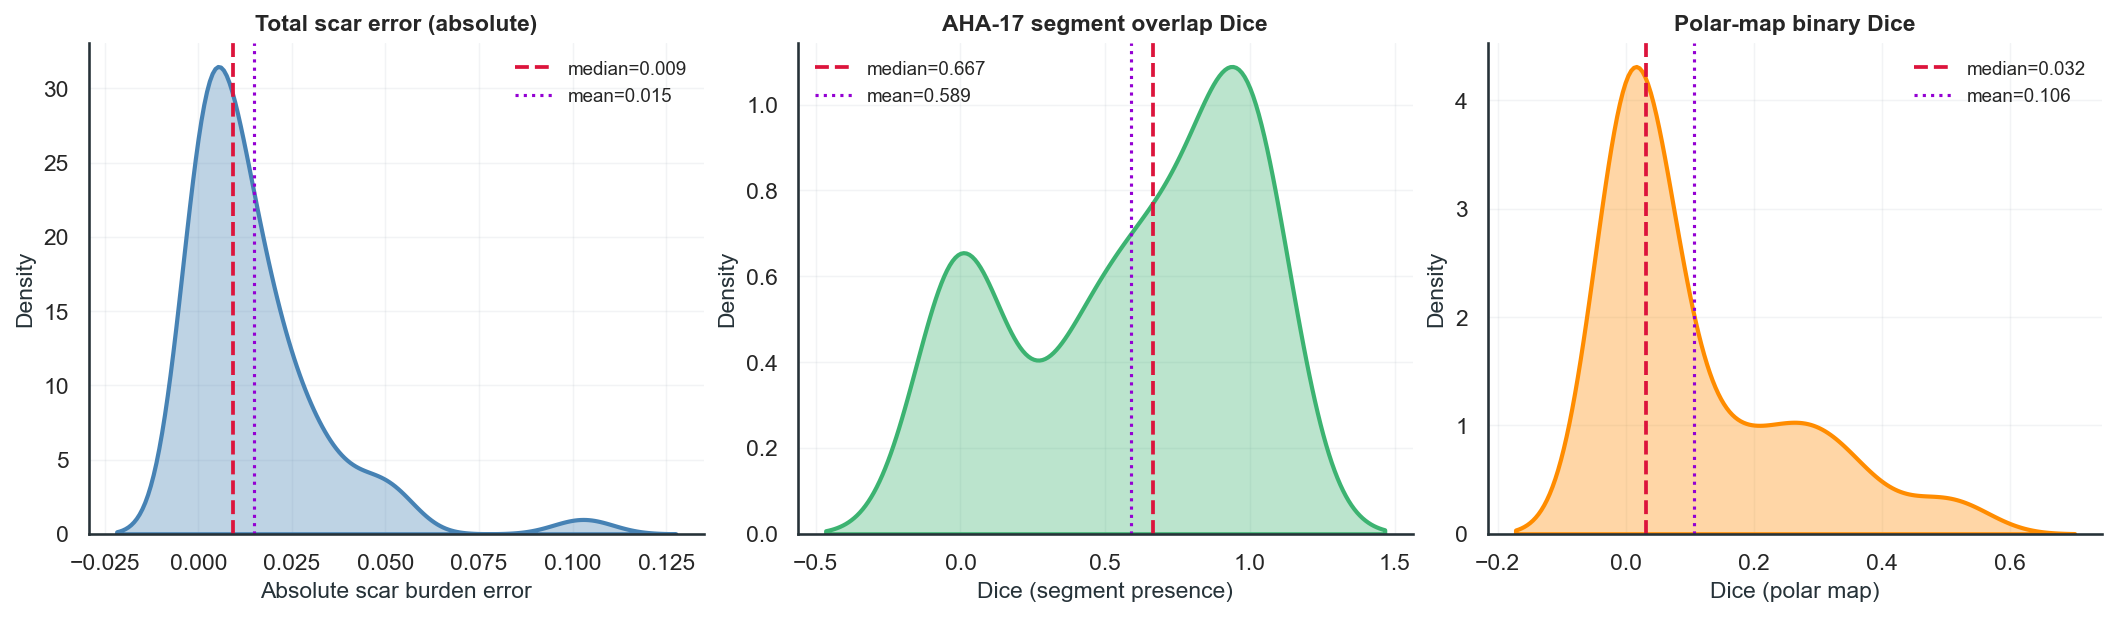
\includegraphics[width=0.70\textwidth]{figures/loo_error_distributions}
    \caption{LOO metric distributions ($n=105$, full vector, Manhattan). Top: $|\Delta\text{CZ}|$ (mean 0.015, median 0.009). Middle: segment Dice (mean 0.597, median 0.667). Bottom: polar-map Dice (mean 0.106, median 0.032).}
    \label{fig:loostats}
\end{figure}
